%% LyX 2.0.5.1 created this file.  For more info, see http://www.lyx.org/.
%% Do not edit unless you really know what you are doing.
\documentclass[english]{article}
\usepackage[T1]{fontenc}
\usepackage[latin9]{inputenc}
\usepackage{geometry}
\geometry{verbose,tmargin=2cm,bmargin=3cm,lmargin=2cm,rmargin=2cm}
\usepackage{amssymb}

\makeatletter

%%%%%%%%%%%%%%%%%%%%%%%%%%%%%% LyX specific LaTeX commands.
\newcommand{\noun}[1]{\textsc{#1}}

%%%%%%%%%%%%%%%%%%%%%%%%%%%%%% User specified LaTeX commands.
%\usepackage{geometry}[margin=1cm]
\usepackage{multicol}
\usepackage{graphicx}

\makeatother

\usepackage{babel}
\begin{document}

\title{Complex Systems Made Simple\\
Project final report\\
$\begin{array}{ccc}
\star &  & \star\\
 & \star
\end{array}$\\
Generative coupled model for Urban configuration optimisation}


\author{\noun{Juste Raimbault}$^{1,2}$\\
$^{1}$D�partement Humanit�s et Sciences Sociales, Ecole Polytechnique\\
$^{2}$LVMT, Ecole Nationale des Ponts et Chauss�es}
\maketitle
\begin{abstract}
We describe an hybrid agent-based model coupling a cellular automata
and a dynamic network, for the simulation of urban growth. Heterogeneous
aspects of urban systems are taken into account in the sense that
morphologic structure but also functional properties of the city are
implied in the evolution. Classic measures of description and performances
for generated configuration are used to classify and explore generated
patterns, and we also propose an economic evaluation of the structure
using sensitivity of segregation models to spatial configuration.
We can apply the model to a real-world situation, proposing an optimisation
of the repartition of activities in a zoning context.

\bigskip{}
\bigskip{}
\bigskip{}

\end{abstract}
\begin{multicols}{2}


\section{Introduction}

Recent progress in many discipline linked directly or indirectly to
Urban Planning can be interpreted as the development of a ``new urban
science'' as \noun{Batty} stands in \cite{batty2013new}. From agent-based
modeling in quantitative geography, which achievements are reviewed
in \cite{heppenstall2012agent}, and for which the best example of
promising results are the series of Simpop models (\cite{pumain2012multi}),
to other approaches of the field that \noun{Portugali} present as
``Complexity theories of cities'' (\cite{portugali2012book}) that
can involve scientists such as physicists as \noun{Haken} on information
theory (\cite{haken2003face}) or architects as \noun{Hillier} with
Space Syntax theory (\cite{hillier1976space}), the field is broad
but is strongly consistent through the common view of urban systems
as complex systems.


\section{Model description}

Our model is adapted from the work of \noun{Moreno} \& \textit{al}.
(\cite{MBB09,moreno2007conception}), that proposed to integrate network
effects in a CA model for modeling urban morphology. Their aim was
to test the effects of physical proximity on urban shape, introducing
the modeling of urban mobility through a network which evolution is
coupled with the evolution of the urban shape. We generalise the model,
allowing to take into account functional properties of the urban environment.


\subsection{Agents and rules}

The world is a square lattice $(P_{i,j})_{1\leq i,j\leq N}$ constitued
of cells that can be occupied or not (that will be denoted by a function
$\delta(i,j,t)$, time being defined on a standard time scale $\mathbb{T}$
which definition is introduced in \cite{golden2012modeling}, and
for which we will take $\tau\mathbb{N}$, $\tau>0$ to simplify).
Among these fixed agents evolves an euclidian network which agents
are roads: $N(t)=(V(t),E(t))$ whith $V$ finite part of the world
(set of points). At initial time, no cell is occupied and the initial
network is fixed: $N(0)=(V_{0},E_{0})$. In order to translate functional
mechanisms in the growth of the city, we suppose that a part of initial
nodes are city centers $C_{0}$ for each an activity is defined by
$a:C_{0}\rightarrow[|1;a_{max}|]$.

Giving these settings and variables, the evolution of the system for
one time step is the following:
\begin{itemize}
\item New cell values are calculated
\item $N$ new cells are built
\end{itemize}
Note that the process is stochastic since it depends on the random
order on which the new cell are built.


\subsection{Evaluation functions}


\paragraph{Morphology}

We qualify the morphologic structure of a configuration by projecting
on a plan corresponding to the following indicators:
\begin{itemize}
\item The integrated local density, calculated by integration with a norm-p
of the densities in circular neighborhood of each cell (with same
radius parameter as for the run). We have, with $p_{d}\in[1;+\infty[$
\[
D(t)=\left[\frac{1}{\sum_{i,j}\delta(i,j,t)}\cdot\sum_{\delta(i,j,t)\neq0}d(i,j,t)^{p_{d}}\right]^{1/p_{d}}
\]

\item The Moran index, defined in \cite{tsai2005quantifying} and used a
lot in quantitative geography such as in \cite{lenechet:hal-00696445},
is used to quantify the polycentric character of the distribution
of populated cells.
\end{itemize}

\paragraph{Network performance}

Because of the way it evolves, the only loops in the network are the
initial ones. Therefore, it has no sense to evaluate robustess or
clustering coefficient of the network. However, since the generated
network is supposed to simulate the mobility network, we can evaluate
as suggested in \cite{banos2012towards} its performance through its
relative speed, i. e. the quantity of detours it obliges to make.


\paragraph{Functional accessibility}


\paragraph{Economic performance}

It has been shown by \noun{Banos} in \cite{banos2012network} that
the \noun{Schelling} segregation model, a basic model for socio-economic
segregation introduced in \cite{schelling1969models}, was highly
sensitive to the spatial structure in which one can embed it (the
segregation laws are in that case also influenced by spatial proximity).
That justify the use of such a model as an evaluation function for
the spatial structure regarding ``economic performance'', in the
sense of how much does the structure influence segregation. We implement
a model for residential dynamics based on the model proposed in \cite{benenson1998multi}.
The output function is a segregation index calculated on residential
patterns obtained from a distribution of constructed patches. Detailed
description of the model is provided in supplementary material S1.


\section{Results}

The model was implemented in NetLogo 5.2 (\cite{NetLogo}). Plots
and charts are managed with R after export into standardised data
(\cite{R}). Primary treatment of GIS Data (for most hand vectorization
of simple raster data) is handled with QGIS (\cite{QGIS_software}).
See supplementary material S2 for implementation details needed for
exact reproducibility.


\subsection{Generation of urban patterns}


\paragraph{Typical patterns}

Different configurations of the weights allow to generate very different
structures.


\paragraph{Classification of structures}


\subsection{Sensitivity analysis and exploration of the parameter space}

\begin{figure}[h] 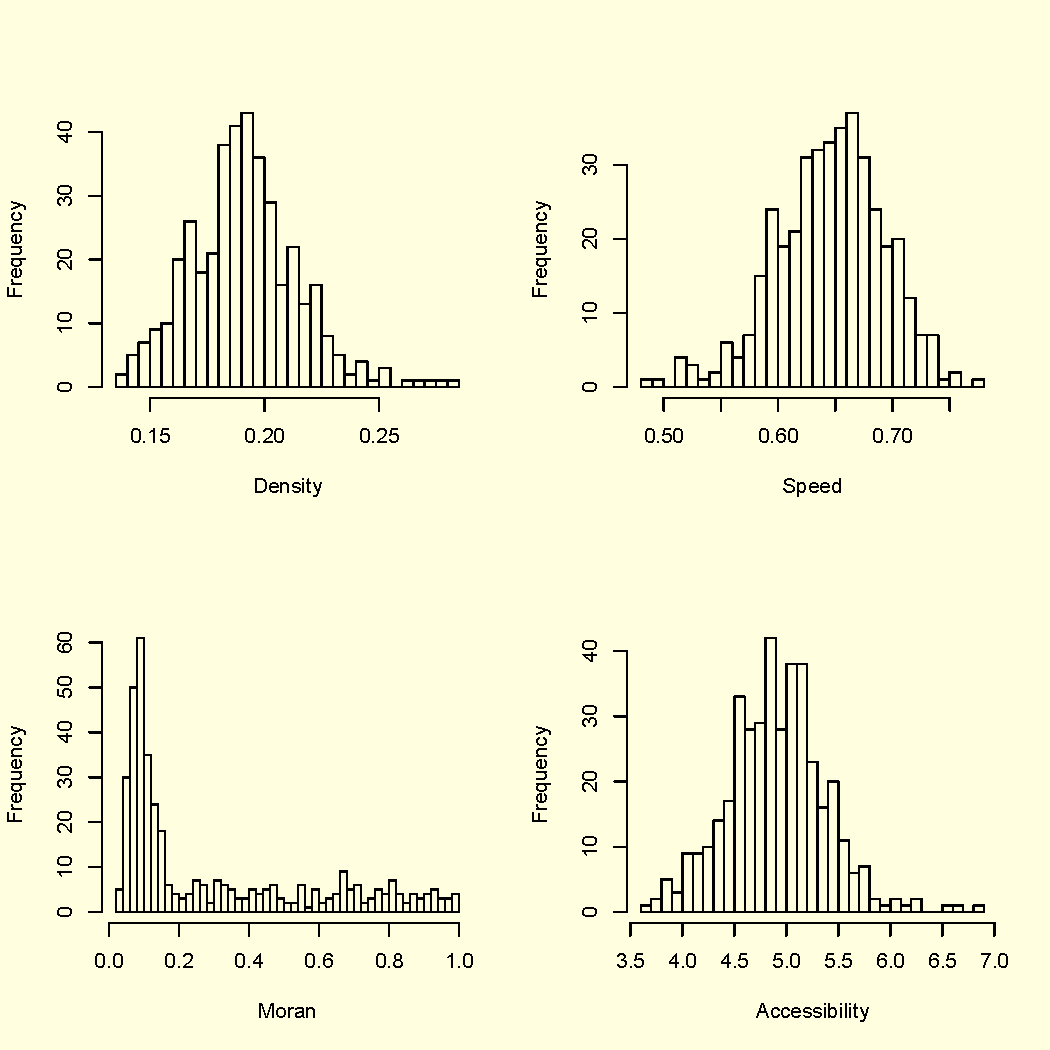
\includegraphics[width=0.3\textwidth]{/Users/Juste/Documents/Cours/ComplexSystemsMadeSimple/project/Results/Robustness/400repets}
\caption{Statistical distribution of outputs for equal weights.}
\end{figure}


\paragraph{Sensitivity to initial conditions}

To determine the magnitude of repetitions useful to get meaningful
values of output functions and to ensure some validity in the results,
it is necessary to investigate the sensitivity of the model to initial
conditions of the spatial configuration. Indeed, if the conclusions
that can be drawn in a particular case are significantly modified
by small changes in the spatial configuration, one will differently
apply the model than in a case where abstract topology of activities
has more influence: one will obviously elaborate totally different
exploration heuristics to proceed to optimisation.

Therefore, we launched large number of simulations with same parameter
values but different initial configurations, in order to get statistical
distributions of outputs at fixed parameters. Standard deviations
were calculated for samples of the parameter space (around 20 samples)
and the distributions were each time of same amplitude and same deviation.
Fig. 3 shows these distributions for the sample corresponding to equal
weights to each parameter. Given the numerical values of deviations
(each time around 0.1 times the amplitude of the function), we can
conclude that outputs are significantly less sensitive to spatial
positions than to topology of activities and parameters values (as
the exploration of parameter space results show in the following).
That justify the small number of repetition needed to have reasonnable
values.


\paragraph{Sensitivity to update type}

The generated structures seem to be quite sensible to the type of
update that is done at each time step, i. e. to the number of cells
that are built at each time step. We can explore a grid of the main
parameter space, 


\paragraph{Exploration of the parameter space}

We explored a grid of the 4-dimensional space of the ``main'' parameters,
the relative weights of variables.


\subsection{Concrete application}

Since we have shown that outputs on which we want to optimise, such
as accessibility to activities or network performance, are significantly
more sensible to initial configuration of activities than to spatial
distribution, we can apply the model to the optimisation of activities
repartition, given an existing spatial structure. That situation can
occur in a planning problem, then one has to decide possible landuses
of predefined zones.


\section{Discussion}

The reproduction of existing urban facts (in the sense of the morphological
structures) and the possible applications showed that the implemented
model may be useful for evidence-based decision-making in urban planning.
However, many aspects can be discussed as they raise crucial questions
and would need further explorations.


\section*{Conclusion}


\section*{Supplementary materials}


\paragraph{S1}

Description of coupled ABM for economic evaluation.


\paragraph{S2}

Core source code of the NetLogo implementation of the model, sample
of data used for applications, source code for generation of plots
and charts.

\bibliographystyle{plain}
\bibliography{/Users/Juste/Documents/Cours/ComplexSystemsMadeSimple/project/Biblio/projetCSMS,/Users/Juste/Documents/ComplexSystems/Biblio/BibTeX/global,/Users/Juste/Documents/ComplexSystems/CCUPD/Biblio/ccupd}


\end{multicols}
\end{document}
